\documentclass[aspectratio=169, 10pt]{beamer}

% ---------- Tema y colores ----------
\usetheme{default}
\usecolortheme{default}
\setbeamertemplate{navigation symbols}{}
\setbeamertemplate{footline}[frame number]
\setbeamertemplate{frametitle continuation}{}

\definecolor{StanfordRed}{RGB}{140,21,21}
\definecolor{StanfordGray}{RGB}{77,77,77}
\definecolor{LightGray}{RGB}{240,240,240}
\definecolor{AccentBlue}{RGB}{0,84,166}
\definecolor{AccentGreen}{RGB}{0,130,100}
\definecolor{UCMBlue}{RGB}{4, 171, 226}
\definecolor{UCMNavy}{RGB}{20, 65, 134}

% Alias de la paleta antigua: las figuras TikZ de esta clase siguen
% usando mitblue/mitgray, que ahora apuntan a los colores UCM.
\definecolor{mitblue}{RGB}{20, 65, 134}
\definecolor{mitgray}{RGB}{169, 169, 169}
\definecolor{backgroundblue}{HTML}{D7EAF3}
\definecolor{catyellow}{HTML}{FCDA76}
\definecolor{catstripe}{HTML}{F9B74C}
\definecolor{yarnred}{HTML}{E26B6B}
\definecolor{bowlblue}{HTML}{66A3D4}
\definecolor{bboxblue}{HTML}{5E69B1}
\definecolor{bboxred}{HTML}{D9534F}
\definecolor{bboxgreen}{HTML}{008000}

\setbeamercolor{frametitle}{fg=white, bg=UCMBlue}
\setbeamercolor{title}{fg=white}
\setbeamercolor{author}{fg=white}
\setbeamercolor{institute}{fg=white!80}
\setbeamercolor{structure}{fg=UCMBlue}
\setbeamercolor{block title}{bg=UCMBlue!15!white, fg=UCMBlue}
\setbeamercolor{block body}{bg=LightGray}
\setbeamercolor{block title alerted}{bg=StanfordRed!15!white, fg=StanfordRed}
\setbeamercolor{block body alerted}{bg=LightGray}
\setbeamercolor{block title example}{bg=AccentGreen!15!white, fg=AccentGreen}
\setbeamercolor{block body example}{bg=LightGray}
\setbeamercolor{alerted text}{fg=UCMBlue}
\setbeamercolor{example text}{fg=UCMBlue}

\setbeamerfont{frametitle}{series=\bfseries, size=\large}
\setbeamerfont{title}{series=\bfseries, size=\LARGE}
\setbeamerfont{block title}{series=\bfseries}

% ---------- Paquetes ----------
\usepackage[utf8]{inputenc}
\usepackage[T1]{fontenc}
\usepackage[provide=*,spanish]{babel}
\usepackage{amsmath, amssymb, bm}
\usepackage{graphicx}
\usepackage{tikz}
\usepackage{pgfplots}
\pgfplotsset{compat=1.18}
\usetikzlibrary{arrows, arrows.meta, shapes, shapes.geometric, positioning,
	fit, calc, matrix, chains, mindmap, decorations.pathreplacing,
	backgrounds, shadows, patterns}
\usepackage{booktabs}
\usepackage{xcolor}
\usepackage{multicol}
\usepackage{tcolorbox}
\tcbuselibrary{skins, breakable}
\usepackage{tikzlings}


% ---------- Comandos útiles ----------
\providecommand{\R}{\mathbb{R}}
\providecommand{\E}{\mathbb{E}}
\providecommand{\Var}{\operatorname{Var}}
\providecommand{\relu}{\operatorname{ReLU}}

\newcommand{\formula}[1]{%
	\begin{tcolorbox}[colback=UCMBlue!8, colframe=UCMBlue, arc=4pt,
		boxsep=2pt, left=6pt, right=6pt, top=3pt, bottom=3pt]
		#1
	\end{tcolorbox}
}

% ---------- Portada ----------
\title{\textbf{Visi\'on Computacional}}
\subtitle{Tareas, im\'agenes y transformaciones}
\author{Sergio Hern\'andez, PhD\\ shernandez@ucm.cl}
\institute{
	\begin{tikzpicture}[scale=0.42, every node/.style={transform shape}]
		\foreach \i/\y in {1/0,2/1,3/2}{\node[circle,draw=white,fill=white!20,minimum size=4mm] (i\i) at (0,\y){};}
		\foreach \i/\y in {1/-0.5,2/0.5,3/1.5,4/2.5}{\node[circle,draw=white,fill=white!35,minimum size=4mm] (h\i) at (2,\y){};}
		\foreach \i/\y in {1/0.5,2/1.5}{\node[circle,draw=white,fill=white!50,minimum size=4mm] (o\i) at (4,\y){};}
		\foreach \a in {1,2,3}\foreach \b in {1,2,3,4}{\draw[white,opacity=0.5] (i\a)--(h\b);}
		\foreach \a in {1,2,3,4}\foreach \b in {1,2}{\draw[white,opacity=0.5] (h\a)--(o\b);}
	\end{tikzpicture}
	\\ \textbf{Mag\'ister en Data Science --- Universidad Cat\'olica del Maule}}
\date{}


\begin{document}
% --- Título ---
{
	\setbeamertemplate{background}{
		\begin{tikzpicture}[remember picture, overlay]
			\fill[UCMBlue] (current page.south west) rectangle (current page.north east);
			\fill[UCMBlue!70!black, opacity=0.5]
			(current page.south west) -- ++(0,3) -- ++(18,0) -- cycle;
			\foreach \i in {1,...,40}{
				\fill[white, opacity=0.04]
				({random()*17}, {random()*10}) circle ({random()*0.3});
			}
		\end{tikzpicture}
	}
	\begin{frame}[plain]
		\vspace{1.2cm}
		\titlepage
		\begin{tikzpicture}[remember picture, overlay]
			\node[white, opacity=0.15, font=\fontsize{80}{80}\selectfont]
			at (current page.east) [xshift=-2cm] {$\mathcal{I}$};
		\end{tikzpicture}
	\end{frame}
}

\section{Introducci\'on}
% --- Diapositiva 1: Introducción ---
% =================================================================
% SECCIÓN 1: OPTIMIZACIÓN
\begin{frame}[fragile]
	\frametitle{Tipos de Problemas en Visión Computacional}
	
	\begin{figure}
		\centering
		\resizebox{\textwidth}{!}{%
			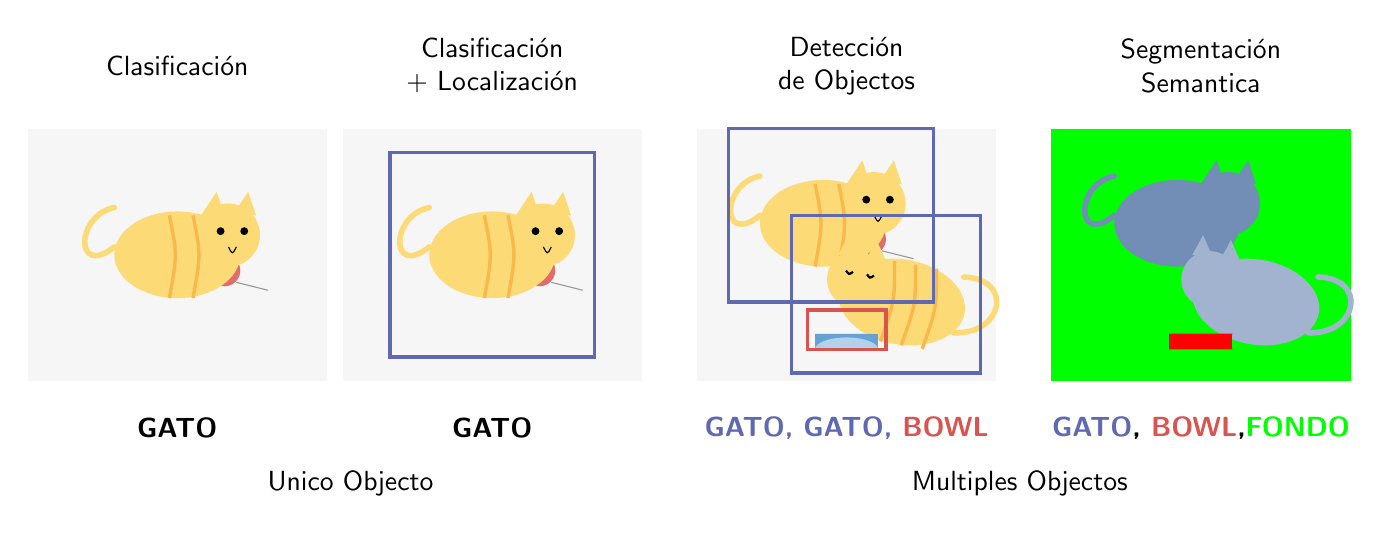
\begin{tikzpicture}[
				font=\sffamily,
				% Estilo para el fondo de cada "imagen"
				imagebg/.style={
					rectangle, 
					fill=mitgray!10, 
					minimum width=3.8cm, 
					minimum height=3.2cm
				},
				% Estilo para los títulos de cada sección
				titlestyle/.style={
					align=center, 
					font=\sffamily,
					text width=3cm
				},
				% Estilo para las etiquetas debajo de las imágenes
				labelstyle/.style={
					align=center, 
					font=\sffamily\bfseries
				},
				% Estilo para las cajas delimitadoras (bounding boxes)
				bbox/.style={draw=bboxblue, very thick},
				bbox-red/.style={draw=bboxred, very thick}
				]
				
				
				% --- Definición de los elementos gráficos para reutilizarlos ---
				
				% Gato 1 (sentado, jugando)
				\newcommand{\catone}[1]{
					\begin{scope}[#1]
						% Ovillo de lana
						\fill[yarnred] (0.6, -0.2) circle (0.2cm);
						\draw[black!40] (0.75, -0.35) -- +(0.4, -0.1);
						% Cola
						\draw[catyellow, line width=2pt, cap=round] 
						(-0.8, 0.1) .. controls (-1.3, -0.3) and (-1.3, 0.5) .. (-0.8, 0.6);
						% Cuerpo
						\fill[catyellow] (0,0) ellipse (0.8cm and 0.55cm);
						% Cabeza
						\fill[catyellow] (0.65, 0.25) circle (0.4cm);
						% Rayas
						\foreach \y in {-0.1, 0.2} {
							\draw[catstripe, line width=1.2pt] (\y,0.5) .. controls (\y+0.1,0) .. (\y, -0.55);
						}
						% Orejas
						\fill[catyellow] (0.3, 0.5) -- (0.5, 0.8) -- (0.6, 0.5) -- cycle;
						\fill[catyellow] (0.7, 0.5) -- (0.9, 0.8) -- (1.0, 0.5) -- cycle;
						% Ojos y boca
						\fill (0.55, 0.3) circle (0.05cm); \fill (0.85, 0.3) circle (0.05cm);
						\draw (0.65, 0.1) .. controls (0.7, 0.0) .. (0.75, 0.1);
					\end{scope}
				}
				\newcommand{\catonemask}[1]{
					\begin{scope}[#1]
						% Ovillo de lana
						%\fill[yarnred] (0.6, -0.2) circle (0.2cm);
						%\draw[black!40] (0.75, -0.35) -- +(0.4, -0.1);
						% Cola
						\draw[mitblue!60, line width=2pt, cap=round] 
						(-0.8, 0.1) .. controls (-1.3, -0.3) and (-1.3, 0.5) .. (-0.8, 0.6);
						% Cuerpo
						\fill[mitblue!60] (0,0) ellipse (0.8cm and 0.55cm);
						% Cabeza
						\fill[mitblue!60] (0.65, 0.25) circle (0.4cm);
						% Orejas
						\fill[mitblue!60] (0.3, 0.5) -- (0.5, 0.8) -- (0.6, 0.5) -- cycle;
						\fill[mitblue!60] (0.7, 0.5) -- (0.9, 0.8) -- (1.0, 0.5) -- cycle;
					\end{scope}
				}
				
				% Gato 2 (junto al cuenco)
				\newcommand{\cattwo}[1]{
					\begin{scope}[#1, scale=0.9, rotate=-10]
						% Cola
						\draw[catyellow, line width=2pt, cap=round] 
						(0.8, -0.3) .. controls (1.5, -0.2) and (1.5, 0.6) .. (0.8, 0.5);
						% Cuerpo
						\fill[catyellow] (0,0) ellipse (0.9cm and 0.6cm);
						% Cabeza
						\fill[catyellow] (-0.7, 0.2) circle (0.4cm);
						% Rayas
						\foreach \y in {-0.2, 0.1, 0.4} {
							\draw[catstripe, line width=1.2pt] (\y,0.55) .. controls (\y+0.1,0) .. (\y, -0.6);
						}
						% Orejas
						\fill[catyellow] (-0.3, 0.5) -- (-0.5, 0.8) -- (-0.6, 0.5) -- cycle;
						\fill[catyellow] (-0.7, 0.5) -- (-0.9, 0.8) -- (-1.0, 0.5) -- cycle;
						% Ojos cerrados
						\draw[thick] (-0.55, 0.3) .. controls (-0.5, 0.25) .. (-0.45, 0.3);
						\draw[thick] (-0.85, 0.3) .. controls (-0.8, 0.25) .. (-0.75, 0.3);
					\end{scope}
				}
				\newcommand{\cattwomask}[1]{
					\begin{scope}[#1, scale=0.9, rotate=-10]
						% Cola
						\draw[mitblue!40, line width=2pt, cap=round] 
						(0.8, -0.3) .. controls (1.5, -0.2) and (1.5, 0.6) .. (0.8, 0.5);
						% Cuerpo
						\fill[mitblue!40] (0,0) ellipse (0.9cm and 0.6cm);
						% Cabeza
						\fill[mitblue!40] (-0.7, 0.2) circle (0.4cm);
						% Orejas
						\fill[mitblue!40] (-0.3, 0.5) -- (-0.5, 0.8) -- (-0.6, 0.5) -- cycle;
						\fill[mitblue!40] (-0.7, 0.5) -- (-0.9, 0.8) -- (-1.0, 0.5) -- cycle;
					\end{scope}
				}
				% Cuenco
				\newcommand{\bowl}[1]{
					\begin{scope}[#1]
						\fill[bowlblue!50!white] (-0.4, 0) arc (180:360:0.4 and 0.15);
						\fill[bowlblue] (-0.4,0) rectangle (0.4, -0.2);
						\fill[bowlblue!50!white] (-0.4, -0.2) arc (180:0:0.4 and 0.15);
					\end{scope}
				}
				\newcommand{\bowlmask}[1]{
					\begin{scope}[#1]
						\fill[red] (-0.4, 0) arc (180:360:0.4 and 0.15);
						\fill[red] (-0.4,0) rectangle (0.4, -0.2);
						\fill[red] (-0.4, -0.2) arc (180:0:0.4 and 0.15);
					\end{scope}
				}
				
				% --- COLUMNA 1: CLASSIFICATION ---
				\begin{scope}[xshift=0cm]
					\node[titlestyle] at (1.6, 4) {Clasificación};
					\node[imagebg] at (1.6, 1.6) {};
					\catone{shift={(1.6,1.6)}};
					\node[labelstyle] at (1.6, -0.6) {GATO};
				\end{scope}
				
				% --- COLUMNA 2: CLASSIFICATION + LOCALIZATION ---
				\begin{scope}[xshift=4cm]
					\node[titlestyle] at (1.6, 4) {Clasificación + Localización};
					\node[imagebg] at (1.6, 1.6) {};
					\catone{shift={(1.6,1.6)}};
					\draw[bbox] (0.3, 0.3) rectangle (2.9, 2.9);
					\node[labelstyle] at (1.6, -0.6) {GATO};
				\end{scope}
				
				% --- COLUMNA 3: OBJECT DETECTION ---
				\begin{scope}[xshift=8.5cm]
					\node[titlestyle] at (1.6, 4) {Detección de Objectos};
					\node[imagebg] at (1.6, 1.6) {};
					\catone{shift={(1.3, 2.0)}};
					\cattwo{shift={(2.3, 1.0)}};
					\bowl{shift={(1.6, 0.6)}};
					% Bounding boxes
					\draw[bbox] (0.1, 1.0) rectangle (2.7, 3.2);
					\draw[bbox] (0.9, 0.1) rectangle (3.3, 2.1);
					\draw[bbox-red] (1.1, 0.4) rectangle (2.1, 0.9);
					\node[labelstyle] at (1.6, -0.6) {\textcolor{bboxblue}{GATO, GATO,} \textcolor{bboxred}{BOWL}};
				\end{scope}
				
				% --- COLUMNA 4: SEMANTIC SEGMENTATION ---
				\begin{scope}[xshift=13cm]
					\node[titlestyle] at (1.6, 4) {Segmentación Semantica};
					\node[imagebg,fill=green] at (1.6, 1.6) {};
					% Máscaras de segmentación
					\catonemask{shift={(1.3, 2.0)} };
					\cattwomask{shift={(2.3, 1.0)} };
					\bowlmask{shift={(1.6, 0.6)} };
					\node[labelstyle] at (1.6, -0.6) {\textcolor{bboxblue}{GATO}, \textcolor{bboxred}{BOWL},\textcolor{green}{FONDO}};
				\end{scope}
				
				% --- ETIQUETAS INFERIORES ---
				\node at (3.8, -1.3) {Unico Objecto};
				\node at (12.3, -1.3) {Multiples Objectos};
				
			
				
			\end{tikzpicture}%
		} % Fin de resizebox
	\end{figure}
	
\end{frame}
\begin{frame}[fragile]
	\frametitle{Clasificación}
	\begin{block}{ ¿A qué categoría o categorías predefinidas pertenece esta imagen?}
		El modelo recibe una imagen como entrada y asigna una etiqueta de una lista de categorías posibles $y_c \in \{0,1,\ldots,K\}$.
	\end{block}
\begin{figure}[h!]
	\centering
		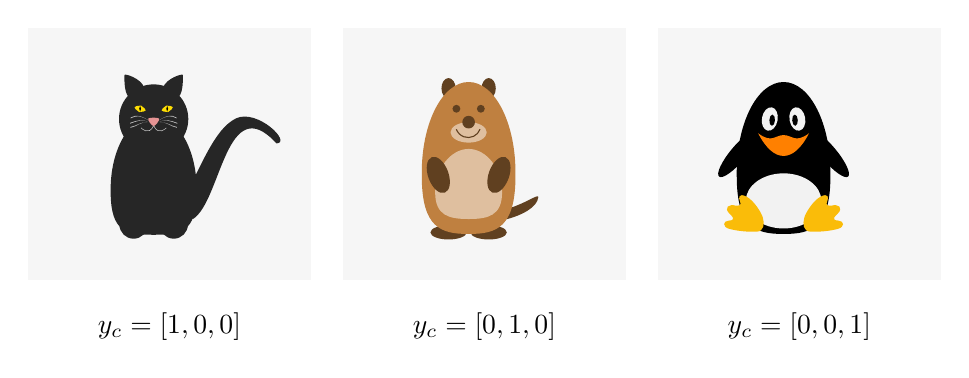
\begin{tikzpicture}[
			font=\sffamily,
			% Estilo para el fondo de cada "imagen"
			imagebg/.style={
				rectangle, 
				fill=mitgray!10, 
				minimum width=3.6cm, 
				minimum height=3.2cm
			},
			% Estilo para los títulos de cada sección
			titlestyle/.style={
				align=center, 
				font=\sffamily,
				text width=3cm
			},
			% Estilo para las etiquetas debajo de las imágenes
			labelstyle/.style={
				align=center, 
				font=\sffamily\bfseries
			},
			% Estilo para las cajas delimitadoras (bounding boxes)
			bbox/.style={draw=bboxblue, very thick},
			bbox-red/.style={draw=bboxred, very thick}
			]
		\begin{scope}[xshift=0cm]
			\node[imagebg] at (1.6, 1.6) {};
			\cat[xshift=1.4cm,yshift=0.4cm];
			\node[labelstyle] at (1.6, -0.6) {$y_c=[1,0,0]$};
		\end{scope}
		
		\begin{scope}[xshift=4cm]
			\node[imagebg] at (1.6, 1.6) {};
			\marmot[xshift=1.4cm,yshift=0.4cm];
			\node[labelstyle] at (1.6, -0.6) {$y_c=[0,1,0]$};
		\end{scope}
		
		\begin{scope}[xshift=8cm]
			\node[imagebg] at (1.6, 1.6) {};
			\penguin[xshift=1.4cm,yshift=0.4cm];
			\node[labelstyle] at (1.6, -0.6) {$y_c=[0,0,1]$};
		\end{scope}
		\end{tikzpicture}

\end{figure}
\end{frame}

\begin{frame}[fragile]
	\frametitle{Clasificación + Localización}
	\begin{block}{¿Cuáles es la ubicación y categoría del objeto en la imagen?}
		El modelo recibe una imagen como entrada y asigna una etiqueta $y_c \in \{0,1,\ldots,K\}$ y una ubicación $y_l \in \mathbb{R}^4$.
	\end{block}
	\begin{figure}[h!]
		\centering
		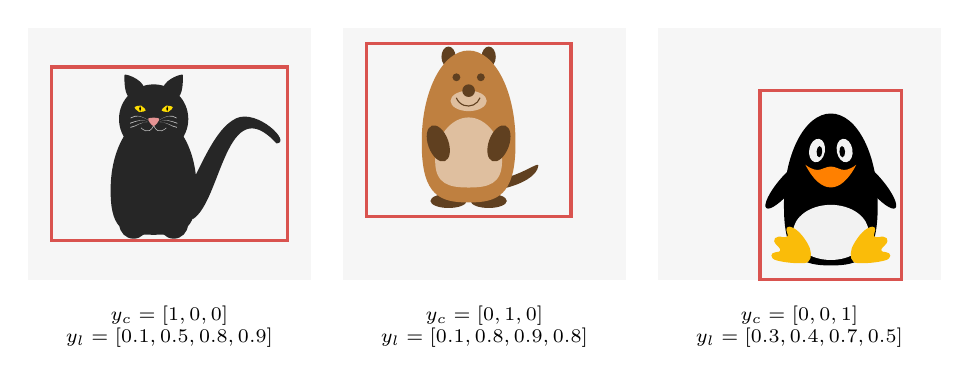
\begin{tikzpicture}[
			font=\tiny,
			% Estilo para el fondo de cada "imagen"
			imagebg/.style={
				rectangle, 
				fill=mitgray!10, 
				minimum width=3.6cm, 
				minimum height=3.2cm
			},
			% Estilo para los títulos de cada sección
			titlestyle/.style={
				align=center, 
				font=\sffamily,
				text width=3cm
			},
			% Estilo para las etiquetas debajo de las imágenes
			labelstyle/.style={
				align=center, 
				font=\sffamily\bfseries\scriptsize
			},
			% Estilo para las cajas delimitadoras (bounding boxes)
			bbox/.style={draw=bboxblue, very thick},
			bbox-red/.style={draw=bboxred, very thick}
			]
			\begin{scope}[xshift=0cm]
				\node[imagebg] at (1.6, 1.6) {};
				\cat[xshift=1.4cm,yshift=0.4cm];
				\draw [bboxred, very thick] (0.1,0.5) rectangle (3.1,2.7);
				\node[labelstyle] at (1.6, -0.6) {$y_c=[1,0,0]$\\$y_l=[0.1,0.5,0.8,0.9]$};
			\end{scope}
			
			\begin{scope}[xshift=4cm]
				\node[imagebg] at (1.6, 1.6) {};
				\marmot[xshift=1.4cm,yshift=0.8cm];
				\draw [bboxred, very thick] (0.1,0.8) rectangle (2.7,3.0);
				\node[labelstyle] at (1.6, -0.6) {$y_c=[0,1,0]$\\$y_l=[0.1,0.8,0.9,0.8]$};
			\end{scope}
			
			\begin{scope}[xshift=8cm]
				\node[imagebg] at (1.6, 1.6) {};
				\penguin[xshift=2cm,yshift=0cm];
				\draw [bboxred, very thick] (1.1,0.0) rectangle (2.9,2.4);
				\node[labelstyle] at (1.6, -0.6) {$y_c=[0,0,1]$\\$y_l=[0.3,0.4,0.7,0.5]$};
			\end{scope}
		\end{tikzpicture}
		
	\end{figure}
\end{frame}

\begin{frame}[fragile]
	\frametitle{Detección de Objetos}
	\begin{block}{¿Cuáles son las ubicaciones exactas de los objetos en la imagen?}
		El modelo no solo clasifica los objetos, sino que también dibuja una \textit{caja delimitadora} (bounding box) alrededor de cada uno para indicar su posición y tamaño.
	\end{block}
	\begin{figure}[h!]
		\centering
		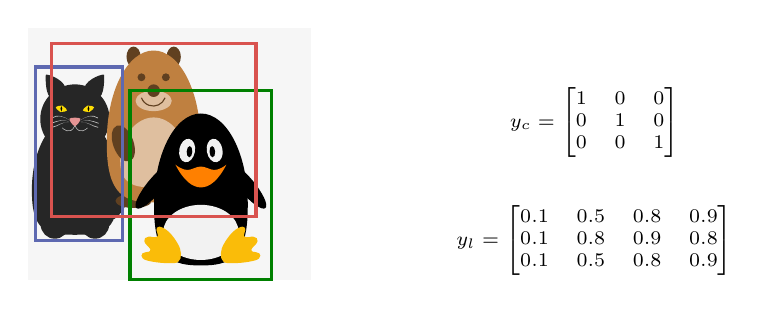
\begin{tikzpicture}[
			font=\tiny,
			% Estilo para el fondo de cada "imagen"
			imagebg/.style={
				rectangle, 
				fill=mitgray!10, 
				minimum width=3.6cm, 
				minimum height=3.2cm
			},
			% Estilo para los títulos de cada sección
			titlestyle/.style={
				align=center, 
				font=\sffamily,
				text width=3cm
			},
			% Estilo para las etiquetas debajo de las imágenes
			labelstyle/.style={
				align=center, 
				font=\sffamily\bfseries\scriptsize
			},
			% Estilo para las cajas delimitadoras (bounding boxes)
			bbox/.style={draw=bboxblue, very thick},
			bbox-red/.style={draw=bboxred, very thick}
			]
			\begin{scope}[xshift=0cm]
				\node[imagebg] at (1.6, 1.6) {};
				\cat[xshift=0.4cm,yshift=0.4cm];
				\marmot[xshift=1.4cm,yshift=0.8cm];
				\penguin[xshift=2cm,yshift=0cm];
				\draw [bboxgreen, very thick] (1.1,0.0) rectangle (2.9,2.4);
				\draw [bboxblue, very thick] (-0.1,0.5) rectangle (1.0,2.7);
				\draw [bboxred, very thick] (0.1,0.8) rectangle (2.7,3.0);
				%\node[labelstyle] at (1.6, -0.6) {$y_c=[1,0,0]$\\$y_l=[0.1,0.5,0.8,0.9]$};
			\end{scope}
			
			\begin{scope}[xshift=5.0cm]
				\node[labelstyle] at (2, 2) {$y_c=\begin{bmatrix}
										1 & 0 & 0\\
										0 & 1 & 0\\
										0 & 0 & 1
										\end{bmatrix}$};
				\node[labelstyle] at (2, 0.5) {$y_l=\begin{bmatrix}
										0.1&0.5&0.8&0.9\\
										0.1&0.8&0.9&0.8\\
										0.1&0.5&0.8&0.9
										\end{bmatrix}$};
			\end{scope}
			
		\end{tikzpicture}
		
	\end{figure}
\end{frame}

\begin{frame}[fragile]
	\frametitle{Segmentación Semántica}
	\begin{block}{¿Cuáles son los límites y la categoría de cada uno de los pixeles?}
		A cada píxel de la imagen se le asigna una categoría. Esto permite una comprensión detallada de la escena, separando los objetos de su entorno con precisión.
		\end{block}
	\begin{figure}[h!]
		\centering
		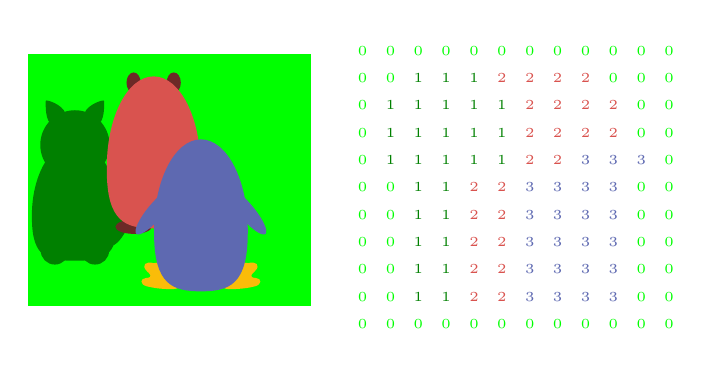
\begin{tikzpicture}[
			font=\tiny,
			% Estilo para el fondo de cada "imagen"
			imagebg/.style={
				rectangle, 
				fill=mitgray!10, 
				minimum width=3.6cm, 
				minimum height=3.2cm
			},
			% Estilo para los títulos de cada sección
			titlestyle/.style={
				align=center, 
				font=\sffamily,
				text width=3cm
			},
			% Estilo para las etiquetas debajo de las imágenes
			labelstyle/.style={
				align=center, 
				font=\sffamily\bfseries\scriptsize
			},
			% Estilo para las cajas delimitadoras (bounding boxes)
			bbox/.style={draw=bboxblue, very thick},
			bbox-red/.style={draw=bboxred, very thick}
			]
			\begin{scope}[xshift=0cm]
				\node[imagebg,fill=green] at (1.6, 1.6) {};
				\cat[back,xshift=0.4cm,yshift=0.4cm,body=bboxgreen];
				\marmot[back,xshift=1.4cm,yshift=0.8cm,body=bboxred];
				\penguin[back,xshift=2cm,yshift=0cm,body=bboxblue];
			\end{scope}
			
			\def\matrixdata{
				{0,0,0,0,0,0,0,0,0,0,0,0},
				{0,0,1,1,1,2,2,2,2,0,0,0},
				{0,1,1,1,1,1,2,2,2,2,0,0},
				{0,1,1,1,1,2,2,2,2,2,0,0},
				{0,1,1,1,1,2,2,3,3,3,3,0},
				{0,0,1,1,2,2,3,3,3,3,3,0},
				{0,0,1,1,2,3,3,3,3,3,3,0},
				{0,0,1,1,2,3,3,3,3,3,3,0},
				{0,0,0,0,2,2,3,3,3,3,0,0},
				{0,0,0,0,0,2,0,3,3,0,0,0},
				{0,0,0,0,0,0,0,0,0,0,0,0},
				{0,0,0,0,0,0,0,0,0,0,0,0}
			}
			\begin{scope}[xshift=6.0cm,yshift=1.5cm]
			  \matrix [matrix of nodes]
			 {
			 	 |[green]| 0& |[green]| 0& |[green]| 0& |[green]| 0&|[green]| 0& |[green]| 0& |[green]| 0& |[green]| 0& |[green]| 0& |[green]| 0& |[green]| 0& |[green]|0 \\
			 	 |[green]|0 & |[green]| 0 & |[bboxgreen]|  1 & |[bboxgreen]|  1 & |[bboxgreen]|  1 & |[bboxred]|  2 & |[bboxred]|  2 & |[bboxred]|  2 & |[bboxred]|  2 & |[green]|  0 & |[green]|  0 & |[green]| 0\\
			 	 |[green]| 0  & |[bboxgreen]| 1  & |[bboxgreen]| 1  & |[bboxgreen]| 1  & |[bboxgreen]| 1 & |[bboxgreen]|1  & |[bboxred]|2  & |[bboxred]| 2 & |[bboxred]|2  & |[bboxred]| 2  & |[green]| 0  & |[green]| 0\\
			 	 |[green]| 0  & |[bboxgreen]| 1  & |[bboxgreen]| 1  & |[bboxgreen]| 1  & |[bboxgreen]| 1 & |[bboxgreen]|1  & |[bboxred]|2  & |[bboxred]| 2 & |[bboxred]|2  & |[bboxred]| 2  & |[green]| 0  & |[green]| 0\\
			 	 |[green]| 0  & |[bboxgreen]| 1  & |[bboxgreen]| 1  & |[bboxgreen]| 1  & |[bboxgreen]| 1 & |[bboxgreen]|1  & |[bboxred]|2  & |[bboxred]| 2 & |[bboxblue]|3  & |[bboxblue]| 3  & |[bboxblue]| 3  & |[green]| 0\\
			 	 |[green]| 0  & |[green]| 0 & |[bboxgreen]| 1  & |[bboxgreen]| 1  & |[bboxred]|2  & |[bboxred]|2   & |[bboxblue]|3  & |[bboxblue]| 3 & |[bboxblue]|3  & |[bboxblue]| 3  & |[green]| 0  & |[green]| 0\\
			 	 |[green]| 0  & |[green]| 0 & |[bboxgreen]| 1  & |[bboxgreen]| 1  & |[bboxred]|2  & |[bboxred]|2   & |[bboxblue]|3  & |[bboxblue]| 3 & |[bboxblue]|3  & |[bboxblue]| 3  & |[green]| 0  & |[green]| 0\\
			 	 |[green]| 0  & |[green]| 0 & |[bboxgreen]| 1  & |[bboxgreen]| 1  & |[bboxred]|2  & |[bboxred]|2   & |[bboxblue]|3  & |[bboxblue]| 3 & |[bboxblue]|3  & |[bboxblue]| 3  & |[green]| 0  & |[green]| 0\\
			 	 |[green]| 0  & |[green]| 0 & |[bboxgreen]| 1  & |[bboxgreen]| 1  & |[bboxred]|2  & |[bboxred]|2   & |[bboxblue]|3  & |[bboxblue]| 3 & |[bboxblue]|3  & |[bboxblue]| 3  & |[green]| 0  & |[green]| 0\\
			 	 |[green]| 0  & |[green]| 0 & |[bboxgreen]| 1  & |[bboxgreen]| 1  & |[bboxred]|2  & |[bboxred]|2   & |[bboxblue]|3  & |[bboxblue]| 3 & |[bboxblue]|3  & |[bboxblue]| 3  & |[green]| 0  & |[green]| 0\\
			 	 |[green]| 0& |[green]| 0& |[green]| 0& |[green]| 0&|[green]| 0& |[green]| 0& |[green]| 0& |[green]| 0& |[green]| 0& |[green]| 0& |[green]| 0& |[green]|0 \\
			 };
			 
				\end{scope}
%			\begin{scope}[xshift=5.0cm]
%				\node[labelstyle] at (2, 2) {$y_c=\begin{bmatrix}
%										0 & 0 & 0 & 0 & 0 & 0 & 0 & 0 & 0 & 1\\
%         0 & 0 & 0 & 0 & 0 & 0 & 0 & 0& 0& 0\\
%         0 & 0 & 0 & 0 & 0 & 0 & 3 & 3 & 3 & 3\\
%         0 & 0 & 2 & 2 & 2 & 2 & 3 & 3 & 3 & 3\\
%         0 & 0 & 2 & 2 & 2 & 2 & 3 & 3 & 3 & 3\\
%         1 & 1 & 2 & 2 & 2 & 2 & 3 & 3 & 3 & 3\\
%         1 & 1 & 2& 2 & 2 & 2& 3 & 3 & 3 & 3\\
%         1 & 1 & 0 & 0 & 0 & 3 & 3 & 3 & 3 & 3\\
%         0 & 0 & 0 & 0 & 0 & 0 & 3 & 3 & 3 & 3\\
%         0 & 0 & 0 & 0 & 0 & 0 & 0 & 0 & 0& 0\\
%										\end{bmatrix}$};
%				
%			\end{scope}
			
		\end{tikzpicture}
		
	\end{figure}
\end{frame}

\begin{frame}[shrink,fragile]
	\frametitle{Representación de Imágenes en la Computadora}
	\begin{itemize}
	\item Las imágenes se transforman en números.
	\item Una imagen digital está compuesta por una cuadrícula de elementos diminutos llamados pixeles.
	\item Para imágenes en escala de grises, cada píxel es un valor de intensidad entre 0 (negro) y 255 (blanco).
		\end{itemize}	

\begin{figure}
		\centering
		\resizebox{0.4\textwidth}{!}{%
		 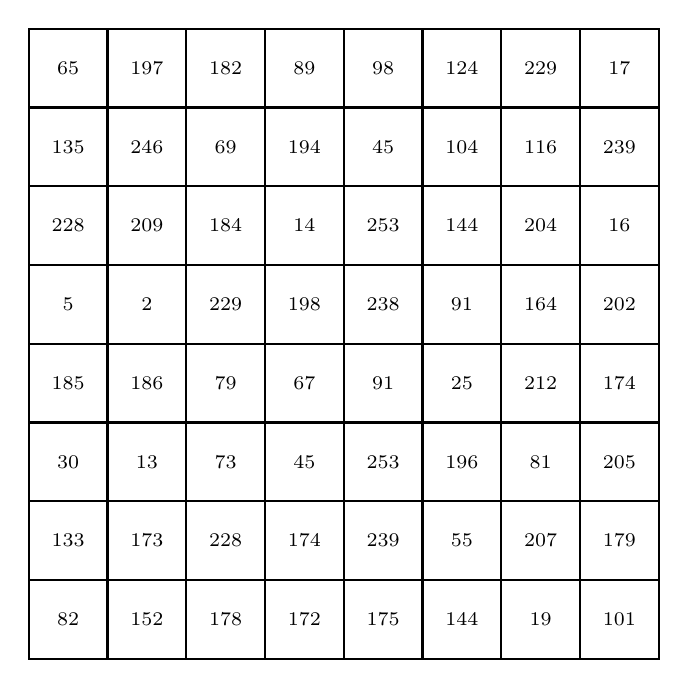
\begin{tikzpicture}
        		\foreach \x in {1,...,8}{
            \foreach \y in {1,...,8}{
                \begin{scope}[shift={(\x,\y)}]
                  \draw[thick]  (0,0) rectangle (1,1);
                  \pgfmathrandominteger{\a}{1}{255};
                  \node[font=\scriptsize] at (0.5, 0.5) {\a};
                \end{scope}
            }
        }
    \end{tikzpicture}
}
\end{figure}
\end{frame}

\begin{frame}[fragile]
	\frametitle{Imágenes a Color}
	\begin{itemize}
	\item Tienen tres canales: Rojo (Red), Verde (Green) y Azul (Blue).
	\item Cada pixel tiene tres valores de intensidad (uno por cada canal), también entre 0 y 255.
	\item La combinación de estos tres valores produce todos los colores visibles. Se pueden crear más de 16 millones de colores.
	\item Una imagen es un tensor de enteros.
		\end{itemize}	

\begin{figure}
		\centering
		\resizebox{\textwidth}{!}{%
		 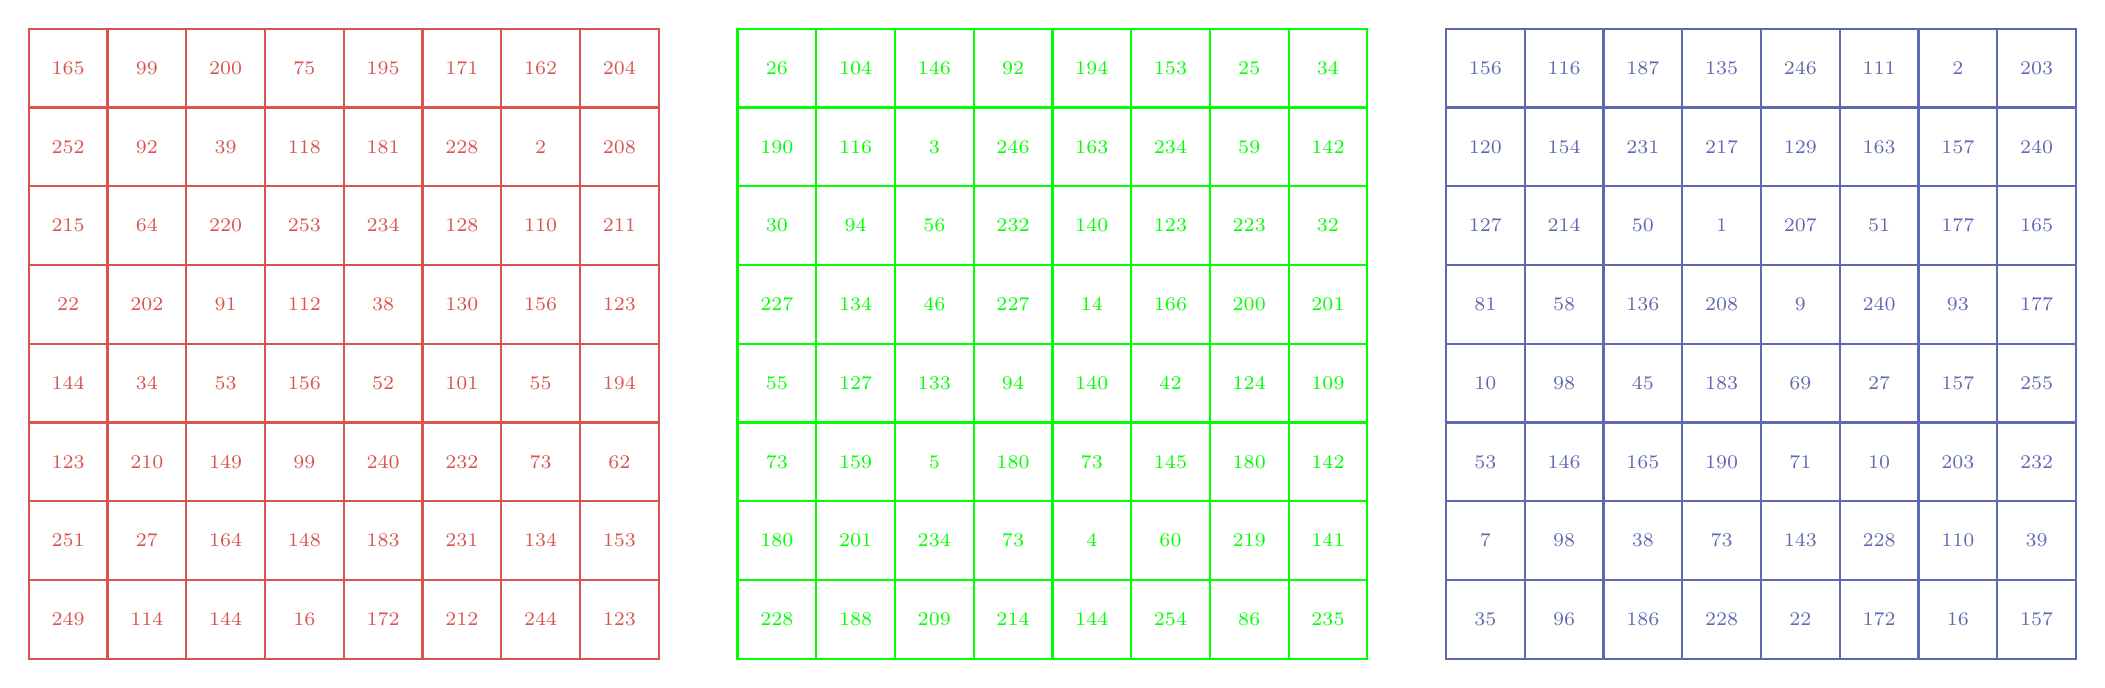
\begin{tikzpicture}
        		\foreach \x in {1,...,8}{
            \foreach \y in {1,...,8}{
                \begin{scope}[shift={(\x,\y)}]
                  \draw[thick,bboxred]  (0,0) rectangle (1,1);
                  \pgfmathrandominteger{\a}{1}{255};
                  \node[font=\scriptsize,color=bboxred] at (0.5, 0.5) {\a};
                \end{scope}
                
                 \begin{scope}[shift={(\x+9,\y)}]
                  \draw[thick,green]  (0,0) rectangle (1,1);
                  \pgfmathrandominteger{\a}{1}{255};
                  \node[font=\scriptsize,color=green] at (0.5, 0.5) {\a};
                \end{scope}
                
                 \begin{scope}[shift={(\x+18,\y)}]
                  \draw[thick,bboxblue]  (0,0) rectangle (1,1);
                  \pgfmathrandominteger{\a}{1}{255};
                  \node[font=\scriptsize,color=bboxblue] at (0.5, 0.5) {\a};
                \end{scope}
            }
        }
    \end{tikzpicture}
}
\end{figure}
\end{frame}

\begin{frame}[shrink,fragile]
	\frametitle{Espacios de Color}
	\begin{itemize}
		\item El espacio de color RGB es aditivo, ya que los colores se obtienen a partir de una combinación lineal de los valores R, G y B.
		\item El espacio de color LAB contiene un canal de información que incluye el brillo (Lightness). Aproxima la forma en que los humanos perciben el color.
		\item HSV es un espacio de color que incluye un canal para la longitud de onda dominante (Hue), mientras los otros canales describen la saturación e intensidad.
	\end{itemize}	
	
\begin{figure}
	\centering
	\resizebox{\textwidth}{!}{%
		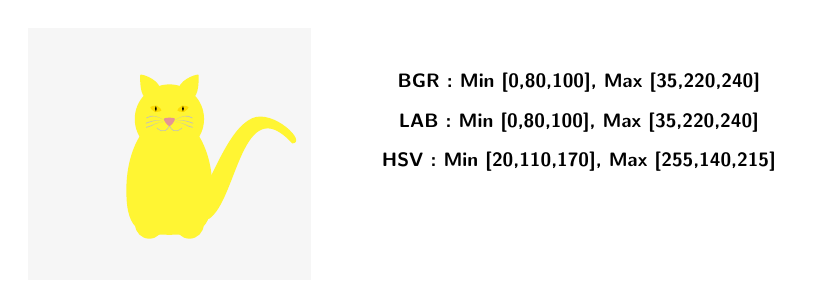
\begin{tikzpicture}[
			font=\tiny,
			% Estilo para el fondo de cada "imagen"
			imagebg/.style={
				rectangle, 
				fill=mitgray!10, 
				minimum width=3.6cm, 
				minimum height=3.2cm
			},
			% Estilo para los títulos de cada sección
			titlestyle/.style={
				align=center, 
				font=\sffamily,
				text width=3cm
			},
			% Estilo para las etiquetas debajo de las imágenes
			labelstyle/.style={
				align=center, 
				font=\sffamily\bfseries\scriptsize
			},
			% Estilo para las cajas delimitadoras (bounding boxes)
			bbox/.style={draw=bboxblue, very thick},
			bbox-red/.style={draw=bboxred, very thick}
			]
		\begin{scope}[xshift=0cm]
			\node[imagebg] at (-1.6, 1.6) {};
			\cat[xshift=-1.6cm,yshift=0.4cm,body=yellow!80];
			\node[labelstyle] at (3.6, 2.5) {BGR : Min [0,80,100], Max [35,220,240]};
			\node[labelstyle] at (3.6, 2.0) {LAB : Min [0,80,100], Max [35,220,240]};
			\node[labelstyle] at (3.6, 1.5) {HSV : Min [20,110,170], Max [255,140,215]};
		\end{scope}
		\end{tikzpicture}
	}
\end{figure}
\end{frame}

\begin{frame}[fragile]
	\frametitle{Traslación}
	\begin{block}{Traslación}
		Corresponde a un desplazamiento de la imagen a lo largo del eje vertical o horizontal. Podemos definir una matriz de traslación como $M=\begin{bmatrix}
			1 & 0 & t_x\\
		0 & 1 & t_y\\
		0 & 0 & 1
		\end{bmatrix}$, que desplaza los elementos de la matriz original $I=\begin{bmatrix}
		x\\
		y\\
		1
		\end{bmatrix}$ en $(x+t_x,y+t_y)$ pixeles.
	\end{block}	
	
	\begin{figure}[h!]
		\centering
		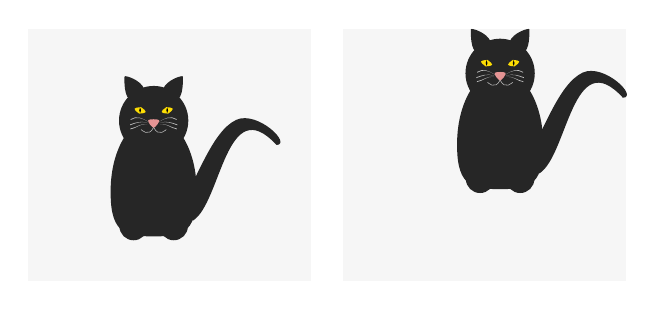
\begin{tikzpicture}[
			font=\sffamily,
			% Estilo para el fondo de cada "imagen"
			imagebg/.style={
				rectangle, 
				fill=mitgray!10, 
				minimum width=3.6cm, 
				minimum height=3.2cm
			},
			% Estilo para los títulos de cada sección
			titlestyle/.style={
				align=center, 
				font=\sffamily,
				text width=3cm
			},
			% Estilo para las etiquetas debajo de las imágenes
			labelstyle/.style={
				align=center, 
				font=\sffamily\bfseries
			},
			% Estilo para las cajas delimitadoras (bounding boxes)
			bbox/.style={draw=bboxblue, very thick},
			bbox-red/.style={draw=bboxred, very thick}
			]
			\begin{scope}[xshift=0cm]
				\node[imagebg] at (1.6, 1.6) {};
				\cat[xshift=1.4cm,yshift=0.4cm];
			\end{scope}
			
			\begin{scope}[xshift=4cm]
				\node[imagebg] at (1.6, 1.6) {};
				\cat[xshift=1.8cm,yshift=1.0cm];
			\end{scope}
			
			
		\end{tikzpicture}
		
	\end{figure}
\end{frame}

\begin{frame}[fragile]
	\frametitle{Rotación}
	\begin{block}{Rotación}
		Corresponde a un desplazamiento de la imagen a lo largo del centro. Podemos definir una matriz de rotación como $M=\begin{bmatrix}
			\cos{\theta} & -\sin{\theta} \\
			\sin{\theta}& \cos{\theta}
		\end{bmatrix}$ aplicada a lo largo del centro de la imagen.
	\end{block}	
	
	\begin{figure}[h!]
		\centering
		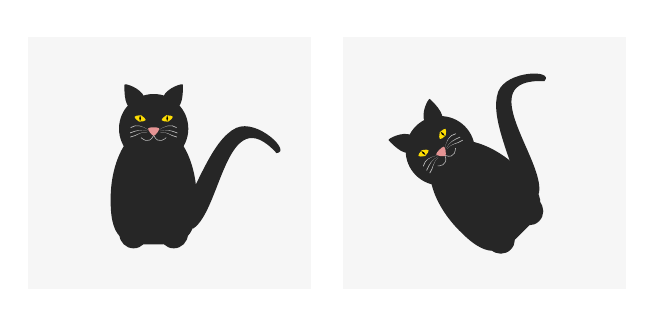
\begin{tikzpicture}[
			font=\sffamily,
			% Estilo para el fondo de cada "imagen"
			imagebg/.style={
				rectangle, 
				fill=mitgray!10, 
				minimum width=3.6cm, 
				minimum height=3.2cm
			},
			% Estilo para los títulos de cada sección
			titlestyle/.style={
				align=center, 
				font=\sffamily,
				text width=3cm
			},
			% Estilo para las etiquetas debajo de las imágenes
			labelstyle/.style={
				align=center, 
				font=\sffamily\bfseries
			},
			% Estilo para las cajas delimitadoras (bounding boxes)
			bbox/.style={draw=bboxblue, very thick},
			bbox-red/.style={draw=bboxred, very thick}
			]
			\begin{scope}[xshift=0cm]
				\node[imagebg] at (1.6, 1.6) {};
				\cat[xshift=1.4cm,yshift=0.4cm];
			\end{scope}
			
			\begin{scope}[xshift=4cm]
				\node[imagebg] at (1.6, 1.6) {};
				\cat[xshift=2.2cm,yshift=0.6cm,rotate=45];
			\end{scope}
			
			
		\end{tikzpicture}
		
	\end{figure}
	

\end{frame}

\begin{frame}[fragile]
	\frametitle{Escalamiento}
	\begin{itemize}
		\item El escalamiento de imágenes corresponde a un cambio del tamaño (resolución) de la imagen original.
		\item Al escalar hacia imágenes de mayor tamaño, requiere interpolar pixeles. Algunas tecnicas de interpolación usadas son:
		\begin{itemize}
			\item Vecinos mas cercanos (KNN)
			\item Interpolación Lineal
			\item Vecindad de pixeles (Lanczos)
		\end{itemize}
		\item Al escalar hacia imágenes de menor tamaño, requiere sub-muestreo de pixeles y por lo tanto introduce el efecto de \textbf{aliasing}.
	\end{itemize}	
	
	
\end{frame}

\begin{frame}[fragile]
	\frametitle{Escalamiento}
	
\begin{figure}[h!]
	\centering
	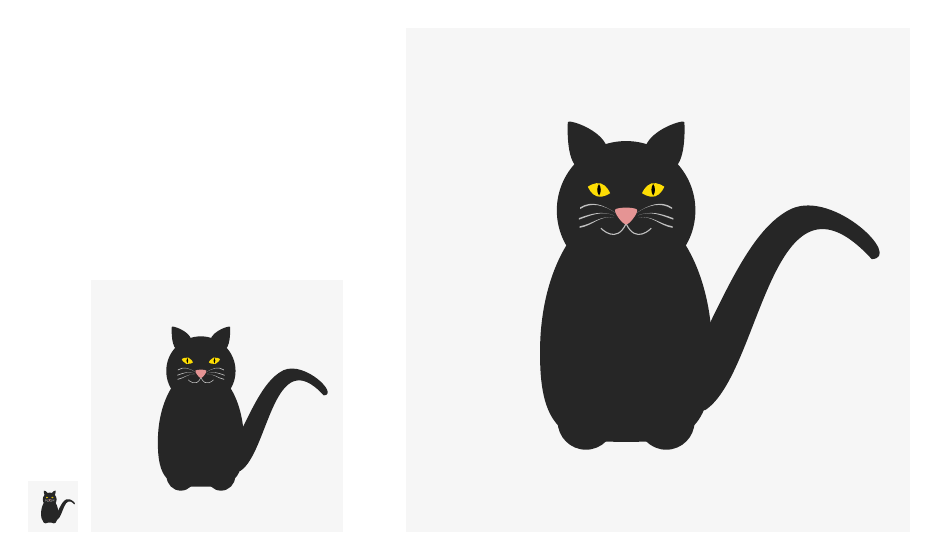
\begin{tikzpicture}[
		font=\sffamily,
		% Estilo para el fondo de cada "imagen"
		imagebg/.style={
			rectangle, 
			fill=mitgray!10, 
			minimum width=3.2cm, 
			minimum height=3.2cm
		},
		% Estilo para los títulos de cada sección
		titlestyle/.style={
			align=center, 
			font=\sffamily,
			text width=3cm
		},
		% Estilo para las etiquetas debajo de las imágenes
		labelstyle/.style={
			align=center, 
			font=\sffamily\bfseries
		},
		% Estilo para las cajas delimitadoras (bounding boxes)
		bbox/.style={draw=bboxblue, very thick},
		bbox-red/.style={draw=bboxred, very thick}
		]
		\begin{scope}[xshift=-0.8cm,scale=0.2]
			\node[imagebg,scale=0.2] at (1.6, 1.6) {};
			\cat[xshift=1.4cm,yshift=0.4cm];
		\end{scope}
		\begin{scope}[xshift=0cm]
			\node[imagebg] at (1.6, 1.6) {};
			\cat[xshift=1.4cm,yshift=0.4cm];
		\end{scope}
		
		\begin{scope}[xshift=4cm,scale=2]
			\node[imagebg,scale=2] at (1.6, 1.6) {};
			\cat[xshift=1.4cm,yshift=0.4cm];
		\end{scope}
		
		
	\end{tikzpicture}
	
\end{figure}
	
\end{frame}


\begin{frame}
	\frametitle{Conclusiones}
	\begin{itemize}
		\item Las imágenes puedes ser almacenadas en un computador como tensores.
		\item Los distintos espacios de color proveen mecanismos que incorporan la percepción humana.
		\item Distintas transformaciones lineales pueden ser usadas para \textit{aumentar} las bases de datos para realizar tareas como la clasificación, detección o segmentación semántica. 
	\end{itemize}	
	
	
\end{frame}
\end{document}